%  ========================================================================
%  Copyright (c) 1985 The University of Washington
%
%  Licensed under the Apache License, Version 2.0 (the "License");
%  you may not use this file except in compliance with the License.
%  You may obtain a copy of the License at
%
%      http://www.apache.org/licenses/LICENSE-2.0
%
%  Unless required by applicable law or agreed to in writing, software
%  distributed under the License is distributed on an "AS IS" BASIS,
%  WITHOUT WARRANTIES OR CONDITIONS OF ANY KIND, either express or implied.
%  See the License for the specific language governing permissions and
%  limitations under the License.
%  ========================================================================
%

% Documentation for University of Washington thesis LaTeX document class
% by Jim Fox
% fox@washington.edu
%
%    Revised 2020/02/24, added \caption()[]{} option.  No ToC.
%
%    Revised for version 2015/03/03 of uwthesis.cls
%    Revised, 2016/11/22, for cleanup of sample copyright and title pages
%
%    This document is contained in a single file ONLY because
%    I wanted to be able to distribute it easily.  A real thesis ought
%    to be contained on many files (e.g., one for each chapter, at least).
%
%    To help you identify the files and sections in this large file
%    I use the string '==========' to identify new files.
%
%    To help you ignore the unusual things I do with this sample document
%    I try to use the notation
%       
%    % --- sample stuff only -----
%    special stuff for my document, but you don't need it in your thesis
%    % --- end-of-sample-stuff ---


%    Printed in twoside style now that that's allowed
%
 
\documentclass [11pt, proquest] {uwthesis}[2020/02/24]

%% VTC additions --------------------------------
\usepackage[
backend=biber,
style=numeric-comp,
% style=authoryear,
% sorting=nyt,
sorting=none,
url=false,
maxbibnames=9,
firstinits=true,
]{biblatex}
\addbibresource{references.bib}

\usepackage{float}
\usepackage{graphicx}
\graphicspath{ {./figures/} }
\usepackage{sidecap}
\usepackage{amsmath}
%--------------------------------
 
%
% The following line would print the thesis in a postscript font 

% \usepackage{natbib}
% \def\bibpreamble{\protect\addcontentsline{toc}{chapter}{Bibliography}}

\setcounter{tocdepth}{1}  % Print the chapter and sections to the toc
 

% ==========   Local defs and mods


%

% --- sample stuff only -----
% These format the sample code in this document

\usepackage{alltt}  % 
\newenvironment{demo}
  {\begin{alltt}\leftskip3em
     \def\\{\ttfamily\char`\\}%
     \def\{{\ttfamily\char`\{}%
     \def\}{\ttfamily\char`\}}}
  {\end{alltt}}
 
% metafont font.  If logo not available, use the second form
%
% \font\mffont=logosl10 scaled\magstep1
\let\mffont=\sf
% --- end-of-sample-stuff ---
 



\begin{document}
 
% ==========   Preliminary pages
%
% ( revised 2012 for electronic submission )
%

\prelimpages
 
%
% ----- copyright and title pages
%
\Title{Wind Waves in Sea Ice of the Western Arctic\\
       and a Global Coupled Wave-Ice Model}
\Author{Vincent T. Cooper}
\Year{2022}
\Program{Atmospheric Sciences}

\Chair{Cecilia Bitz}{Professor and Chair}{Department of Atmospheric Sciences}
\Signature{Kyle Armour}
\Signature{Shuyi Chen}
\Signature{Jim Thomson}

\copyrightpage

\titlepage  

 
%
% ----- signature and quoteslip are gone
%

%
% ----- abstract
%


\setcounter{page}{-1}
\abstract{%
The retreat of Arctic sea ice is enabling increased ocean wave activity at the ice edge, yet the interactions between surface waves and sea ice are not fully understood. Here, we examine in situ observations of wave spectra spanning 2012-2021 in the western Arctic marginal ice zone (MIZ). Swell waves are rarely observed beyond 100 km inside the MIZ. However, local wind waves are observed forming in patches of open water amid partial ice cover during summer. These local waves remain fetch-limited between ice floes with heights less than 1 m. To investigate the physics of these waves, we conduct experiments varying wave attenuation and generation in ice in a global model with coupled interactions between waves and sea ice. A weak high-frequency attenuation rate is required to simulate the wind waves reported in observations. The choice of attenuation scheme and the wind input in ice have a remarkable impact on the extent of wave activity in sea ice across polar oceans, particularly in the Southern Hemisphere. As well as demonstrating the need for stronger constraints on wave attenuation, our results suggest further attention should be paid to locally generated wind waves and their role in sea ice evolution.
% \begin{itemize}
% \item It describes the use of a specialized
% macro package developed specifically for thesis production
% at the University.
% The macros customize \LaTeX\ for the correct thesis style,
% allowing the student to concentrate on the substance of
% his or her text.%
% \footnote{See Appendix A to obtain the source to this
%  thesis and the class file.}
% \item It demonstrates the solutions to a variety of
% formatting challenges found in thesis production.
% \item It serves as a template for a real dissertation.
% \end{itemize}
}
 
%
% ----- contents & etc.
%
\tableofcontents
% \listoffigures
%\listoftables  % I have no tables
 
%
% ----- glossary 
%
% \chapter*{Glossary}      % starred form omits the `chapter x'
% \addcontentsline{toc}{chapter}{Glossary}
% \thispagestyle{plain}
%
% \begin{glossary}
% \item[argument] replacement text which customizes a \LaTeX\ macro for
% each particular usage.
% \item[back-up] a copy of a file to be used when catastrophe strikes
% the original.  People who make no back-ups deserve
% no sympathy.
% \item[control sequence] the normal form of a command to \LaTeX.
% \item[delimiter] something, often a character, that indicates
% the beginning and ending of an argument.
% More generally, a delimiter is a field separator.
% \item[document class] a file of macros that tailors \LaTeX\ for
% a particular document.  The macros described by this thesis
% constitute a document class.
% \item[document option] a macro or file of macros
% that further modifies \LaTeX\ for
% a particular document.  The option {\tt[chapternotes]}
% constitutes a document option.
% \item[figure] illustrated material, including graphs,
% diagrams, drawings and photographs.
% \item[font] a character set (the alphabet plus digits
% and special symbols) of a particular size and style.  A couple of fonts
% used in this thesis are twelve point roman and {\sl twelve point roman
% slanted}.
% \item[footnote] a note placed at the bottom of a page, end of a chapter,
% or end of a thesis that comments on or cites a reference
% for a designated part of the text.
% \item[formatter] (as opposed to a word-processor) arranges printed
% material according to instructions embedded in the text.
% A word-processor, on the other hand, is normally controlled
% by keyboard strokes that move text about on a display.
% \item[\LaTeX] simply the ultimate in computerized typesetting.
% \item[macro]  a complex control sequence composed of 
% other control sequences.
% \item[pica] an archaic unit of length.  One pica is twelve points and
% six picas is about an inch.
% \item[point] a unit of length.  72.27 points equals one inch.
% \item[roman]  a conventional printing typestyle using serifs.
% the decorations on the ends of letter strokes.
% This thesis is set in roman type.
% \item[rule] a straight printed line; e.g., \hrulefill.
% \item[serif] the decoration at the ends of letter strokes.
% \item[table] information placed in a columnar arrangement.
% \item[thesis] either a master's thesis or a doctoral dissertation.
% This document also refers to itself as a thesis, although it
% really is not one.
 
% \end{glossary}
 
%
% ----- acknowledgments
%
\acknowledgments{% \vskip2pc
  % {\narrower\noindent
  I would like to do a $CO_2$ acknowledgment: our emissions of carbon dioxide need to decline.  
  
  
  I would like thank Cecilia Bitz for giving me the opportunity to come to the University of Washington, for her mentorship, and for helping me understand how much I could learn from conducting my own experiments. I had no previous research experience, but she gave me a chance to start fresh and become a scientist. I would like to thank Lettie Roach for being a fantastic mentor, especially when I showed up at UW as nothing but a tabula rasa. I would like to thank Kyle Armour for welcoming me into his research group when I first arrived as a curious character at UW. I would like to thank Greg Hakim for his guidance in broadening my research horizons. I would like to thank Jim Thomson for sharing his expertise on wave-ice interactions, for helping me learn so much along the way, and especially for finding a way for me to do field research in the Arctic Ocean. I would like to thank Shuyi Chen for joining my committee and lending her wave expertise.  
  
  I would like to thank the Arctic Mobile Observing System (AMOS) team, especially Craig Lee, for welcoming me aboard the R/V Sikuliaq. The Arctic is a glorious place. I would also like to thank the UW Program on Climate Change (PCC) for providing a forum where science can be social. I thank the United States of America Department of Defense for funding support through a National Defense Science \& Engineering Graduate (NDSEG) Fellowship.
  % \par}
}

%
% ----- dedication
%
% \dedication{\begin{center}to my dear wife, Joanna\end{center}}

%
% end of the preliminary pages
 
 
 
%
% ==========      Text pages
%

\textpages
 
% ========== Chapter 1
 
\chapter {Introduction}
 
% general intro - why should we care about this topic
As sea ice retreats and exposes larger open water areas in the Arctic Ocean, interactions between ocean surface waves and sea ice may play an elevated role in the Arctic climate system \cite{Thomson2014SwellOcean}. Wave-ice interactions typically occur in the marginal ice zone (MIZ), the partially ice-covered region that separates interior pack ice from open ocean. The fracture of sea ice by ocean surface waves in the MIZ may affect regional climate feedbacks through enhanced sea ice melt (e.g. \cite{Asplin2012FractureStorms}) motivating the development of fully coupled wave-ice models in recent years (e.g. \cite{Roach2019, Boutin2020TowardsZone}).  

However, significant uncertainty remains in our understanding of fundamental aspects of wave-ice physics \cite{Shen2022waveice, Thomson2022WaveSystem}. A major obstacle is that observations of waves in polar oceans are rare and hard to obtain, and existing in situ datasets sample a limited range of ocean and sea ice conditions \cite{Collins2015InZone}. Despite recent progress (e.g. \cite{Brouwer2021}), comprehensive datasets from remote sensing are not yet available. These observing challenges leave us with only weak constraints on the ocean surface wave climate within sea ice.  

Swell, low-frequency ocean surface waves that have developed in open ocean areas, can propagate inside the MIZ, decaying with distance from the sea ice edge. Many studies have considered the attenuation of swell waves in sea ice, but theory has not yet converged on a single explanation \cite{Squire2020OceanReappraisal}. A wide variety of attenuation schemes have been proposed based on different theoretical frameworks and/or observations (see \cite{Perrie2022RepresentationsModels}), and their respective impacts on wave climate have not yet been systematically investigated.

% intro to swell versus wind waves
%In open water, wave heights in the Beaufort Sea have been increasing \cite{Wang2015Historical19712013, Liu2016WindAltimeters}. These increases have been attributed to increased fetch, the open water distance available for wave development, which has expanded due to seasonal sea ice loss \cite{Thomson2016EmergingSeas}. However, the open water region outside of the sea ice edge is not the only area where waves may develop. During the summer melt, Arctic sea ice is becoming less compact \cite{Martin2014SeasonalityModel, Thomson2018OverviewProgram, Squire2020OceanReappraisal}, and it is possible that small waves could develop locally in regions of partial ice cover \cite{Masson1989SpectralField, Smith2016} and contribute to ice break-up and lateral melt \cite{Kohout2008AnZone, Asplin2012FractureStorms, Horvat2016InteractionMelting}.  

% what has been done on attenuation
%Many recent studies have focused on the propagation and attenuation of swell, the low-frequency ocean surface waves that have traveled outside of their original wind-generation area, in sea ice (e.g. \cite{Kohout2014Storm-inducedExtent, Li2015ComparisonConditions}, and collated in \cite{Rogers2021EstimatesInversion}). Theory, though, has not yet converged on a single explanation for wave attenuation in ice \cite{Squire2020OceanReappraisal}. A wide variety of attenuation schemes have been proposed based on different theoretical frameworks and observations \cite{Shen2022waveice, Perrie2022RepresentationsModels}, and their respective impacts on wave climate have not yet been systematically investigated.  

% what has been done on wave generation
Besides propagation of swell, ocean surface waves may also be generated inside the sea ice edge by local winds. In contrast to the large body of work on the attenuation of swell and its incorporation in numerical models, less focus has been placed on these high-frequency wind waves. According to \cite{Squire1980}, wind waves tend to dissipate during their first 10-20 km of travel into the sea ice field. However, \cite{Masson1989SpectralField} developed a model explaining how local wind waves can be generated anew in areas of low sea ice concentration (SIC) and sparse ice floes. Using surface buoy measurements, \cite{Smith2016} found support for the open water distance between floes as a control parameter for local wave energy. We are not aware of theories that explain how wind input for wave growth is modified in partial ice cover. The simple assumption in current wave models scales the wind input by the open water fraction \cite{Liu2020SpectralDecay}. The nonlinear transfer that affects wave development is also highly uncertain in sea ice \cite{Rogers2016DissipationSea, Polnikov2007CalculationIce}. As a result, the importance of local wind wave generation in partial ice cover for the Arctic system remains unclear.  

% our work
Here, we leverage multi-year in situ observations from two recent field campaigns in the Western Arctic: the Beaufort Gyre Observing System (BGOS) and Stratified Ocean Dynamics in the Arctic (SODA). In contrast to previous case study approaches, these data from subsurface moorings offer a long-term view of fundamental properties of waves in ice. We examine the significant wave heights, wave spectra, and the prevalence of wind waves and swell in ice. We then compare the wave spectra to results from new experiments in a global coupled wave-ice model \cite{Roach2019}. Because the expected model error in ice-edge position in a coupled, global simulation precludes point-by-point comparison with individual observations, here we evaluate the general character of waves in the model relative to the measurements. We conduct a series of sensitivity experiments to investigate how different wave-ice physics, specifically the attenuation rate and the dependency of wind input on SIC, impacts (i) the comparison of modelled wave spectra with BGOS and SODA data and (ii) the wave climate in sea ice across the polar oceans. While BGOS and SODA observations are confined to the western Arctic, the model can be used to explore wave-ice interactions and their potential significance for sea ice across the global domain.  

The paper is structured as follows. We describe the observations from BGOS and SODA in section \ref{obs} and the coupled wave-ice model in section \ref{model}. We present results from the observations grouped by distance inside the ice edge ($\Delta^{\mathrm{dist}}$) in section \ref{obs-results}. In section \ref{model-results}, we compare results from wave-ice model sensitivity experiments with observations, and in section \ref{model-waveextent}, we explore how varying wave-ice physics affects the wave climate in sea ice across both hemispheres. In section \ref{discussion}, we discuss implications for summer ice melt and future modelling efforts. We conclude in section \ref{conclusion}.  

 
% ========== Chapter 2
\chapter{Methods}\label{sec:meth}
 
\section{In Situ Observations} \label{obs}



We use subsurface-mooring observations obtained from two separate field campaigns:
\begin{enumerate}
    \item The Beaufort Gyre Observing System (BGOS) \cite{Krishfield2014DeteriorationCycle}. BGOS includes two subsurface moorings with upward-looking Nortek Acoustic Wave and Current (AWAC) instruments for surface tracking. BGOS-A and BGOS-D sample every hour and began collecting measurements in 2012 and 2013, respectively. Raw data are processed into wave spectra following \cite{Herbers2012ObservingBuoys, Kuik1988AData, Thomson2018MeasurementsVehicle} as in \cite{Thomson2014SwellOcean, Smith2016}. BGOS data are mostly continuous from 2012-2020 \cite{Thomson2020Long-termSea}.  
    \item The Stratified Ocean Dynamics in the Arctic project (SODA). Three subsurface moorings use the upward-looking Nortek Signature Doppler profiler for acoustic surface tracking. Raw data from SODA are quality-controlled using methods comparable to the BGOS methods, producing measurements of surface wave spectra sampled every two hours. SODA data span 2018-2019 \cite{Brenner2021ComparingSea}.
\end{enumerate}

\begin{table}[!h]
\caption{Summary of In Situ Observations}
\centering
\begin{tabular}{l l l c r r r}
  \hline
  Dataset     & Instrument      & Period      & Lat. Lon. & Open Water$^1$ & 0-100 km$^1$ & 100+ km$^1$ \\
  \hline
  BGOS-A      & AWAC           & 2012-21   & 75N 150W  & 5796 &  54  & 70                  \\
  BGOS-D      & AWAC           & 2013-20   & 74N 140W  & 2481 & 131  &  6                  \\
  SODA-A      & Signature500   & 2018-19   & 73N 148W  & 1096 &  39  & 10                  \\
  SODA-B      & Signature500   & 2018-19   & 75N 146W  &  314 &  97  &  1                  \\
  SODA-C      & Signature500   & 2018-19   & 78N 139W  &    0 &   0  & 11                  \\
%   SWIFTs$^2$  & Buoy         & Oct-Nov 2015& various        & 838                  & 22                  \\
  \hline
  \multicolumn{4}{l}{BGOS-SODA Total} & 9687 & 321 & 98 \\
  \hline 
  \multicolumn{7}{l}{$^1$Count of valid wave measurements in sample with significant wave height exceeding the}\\
  \multicolumn{7}{l}{\hspace{5 pt}0.3 m approximate detection limit; data are grouped by distance inside the ice}\\
  \multicolumn{7}{l}{\hspace{5 pt}edge ($\Delta^{\mathrm{dist}}$), defined in section \ref{distance-method}.}\\
%   \multicolumn{6}{l}{}\\
%   \multicolumn{6}{l}{$^2$Represents 27 buoy deployments}\\
\end{tabular}
\label{tab:obs}
\end{table} 

The aggregate dataset (denoted BGOS-SODA) spans 2012-2021 and five locations in the central Beaufort Sea (Table \ref{tab:obs}, Figure \ref{fig:distance}). Both sets of subsurface moorings detect surface gravity waves via altimeter measurements of surface displacement. A nuance of the moorings (compared to surface buoys, for example) is that the moorings' surface tracking simultaneously measures surface gravity waves and sea ice draft. The spectral signal from surface waves can be distinguished from that of the sea ice bottom during the quality-control process (additional details included in Appendix \ref{icespectra}), ensuring that the ocean wave data represent surface waves, not ice draft.  

\section{Coupled Wave-Ice Model Experiments} \label{model}

We conduct a series of experiments using the CICE5 sea ice model \cite{Hunke2015CICE:LA-CC-06-012} coupled to the WAVEWATCH III v5.16 ocean surface wave model (WW3) \cite{TheWAVEWATCHIIIRDevelopmentGroupWW3DG2016User5.16} by \cite{Roach2019}. Instead of taking ice conditions as an input and only predicting the waves (as in operational wave forecasts), both the ice and wave conditions are freely evolving on a global domain. The global coupled wave-sea ice model is forced by the JRA-55 atmospheric reanalysis \cite{KOBAYASHI2015TheCharacteristics, cisl_rda_ds628.0} and coupled to a slab ocean model \cite{Bitz2012Climate4}, which includes annually periodic ocean surface currents. CICE5 is modified to treat the joint floe size and thickness distribution (FSTD) as in \cite{Roach2018AnModel, Roach2019}. The integral of the FSTD over all thicknesses is the FSD, which evolves prognostically subject to lateral growth and melt, welding of floes in freezing conditions, wave-induced floe fracture (following \cite{Horvat2015}) and wave-dependent new ice formation \cite{Roach2018AnModel,Roach2019}.  

The sea ice and wave models are on a displaced-pole nominal 1$^\circ$ grid (gx1v7), and the size of model grid cells near observations in the Beaufort Sea is approximately 50x50 km. This model is the same as FSD-WAVEv2 in \cite{Roach2019}, except here (i) we use a higher wave-sea ice coupling frequency, exchanging the wave spectrum and sea ice concentration, thickness, and mean floe size every hour to better resolve short-timescale wave-ice interactions; (ii) we modify the numerical approach such that the source term for wave-ice interactions in WW3 ($S_{ice}$) is applied alongside the other source terms without time-splitting; and (iii) we use WIFF1.0 \cite{Horvat2022WIFF1.0:Fracture} for floe fracture, which is a computationally efficient version of the \cite{Horvat2015} parameterization developed using machine learning. The model spin-up period covers 2000-2018, and sensitivity experiments with varied attenuation schemes are run for 1 year each, branched from the spin-up at 01 January 2018. We analyze hourly output from 2018, which is during the BGOS-SODA observing period and enables comparisons between the model and observations from the western Arctic.  
%Because the experiments simulate across a global domain, we are able to investigate results in the Northern and Southern Hemispheres.   

The experiments (Table \ref{tab:experiments}) test a wide range of attenuation rates that vary in how they depend on frequency and on wave/ice attributes (illustrated in SI Figure \ref{SI:alpha}). We test the six IC4 attenuation methods included in WW3 \cite{TheWAVEWATCHIIIRDevelopmentGroupWW3DG2016User5.16, Collins2017ANRL/MR/7320179726}, as well as the attenuation scheme used by \cite{Roach2019} (denoted FSD-scatter). FSD-scatter is an empirical fit to the floe-scattering theory of \cite{Meylan2021AFloes} with a supplemental attenuation term for long wavelengths, and it depends on mean floe size and mean ice thickness. We use FSD-scatter during model spin-up.  
%Details on the IC4 attenuation methods can be found in \cite{TheWAVEWATCHIIIRDevelopmentGroupWW3DG2016User5.16, Collins2017ANRL/MR/7320179726}. %Experiments are summarized in Table \ref{tab:experiments}, and their attenuation rates are illustrated in SI Figure \ref{SI:alpha}.

\begin{table}[!h]
\caption{Summary of Model Experiments (Varying Attenuation Rates)}
\centering
\begin{tabular}{l l l l}
  \hline
  Experiment    & $\alpha$: 2.5 s$^1$  & Ref.   & $\alpha$ Dependencies \\
  \hline
  IC4M1      & $4 \times 10^{-4}$      & \cite{Wadhams1988TheZone} & Period only as exponential function \\
  IC4M2      & $2 \times 10^{-3}$      & \cite{Meylan2014InZone}     & Period only as 4\textsuperscript{th} degree polynomial\\
  IC4M3rad1  & $2 \times 10^{-1}$      & \cite{Horvat2015, Kohout2008AnZone} & Period; ice thickness\textsuperscript{2}\\
  IC4M4      & $1 \times 10^{-5}$      & \cite{Kohout2014Storm-inducedExtent} & Depends only on significant wave height ($H_s$) \\
  IC4M5      & $2 \times 10^{-4}$      & \cite{Collins2017ANRL/MR/7320179726}  & Period only as piecewise step function (Fig. \ref{SI:alpha})\\
  IC4M7      & $1 \times 10^{-2}$      & \cite{Doble2015RelatingResults}   & Period; ice thickness \\
  FSD-scatter      & $5 \times 10^{-3}$   & \cite{Meylan2021AFloes}   & Period; mean floe radius, mean ice thickness \\
  \hline 
  \multicolumn{4}{l}{$^1$Attenuation rate $\alpha$ at high-frequency reference = 0.4 Hz (period $T = 2.5$ s),}\\
  \multicolumn{4}{l}{\ thickness = 0.5 m, significant wave height $H_s$ = 1.0 m (for IC4M4), and}\\
  \multicolumn{4}{l}{\ floe radius = 100 m (for FSD-scatter).}\\
  \multicolumn{4}{l}{$^2 \alpha$ varies with floe radius in \cite{Horvat2015} but has constant radius = 1 m in WW3 \cite{Rogers2021IncorporatingIce}.}\\
  
\end{tabular}
\label{tab:experiments}
\end{table} 

The wave source terms in WW3 are multiplied by SIC (or the open water fraction, $1-SIC$). This default setting reduces the wind input ($S_{in}$) to zero when $SIC=100\%$. Because the effect of ice cover on $S_{in}$ is uncertain, we run an additional set of experiments that allows some wind input to persist when the SIC reaches 100\%. Instead of multiplying $S_{in}$ by the open water fraction $(1-SIC)$, the enhanced wind-input experiments multiply $S_{in}$ by $(1-SIC\mathbf{/2})$. This forces $S_{in}$ to go from its full value to half-strength as SIC goes from zero to 100\%. In all experiments, the nonlinear source is left at its default setting, i.e. it is reduced to zero in 100\% SIC (see discussion in  \cite{Rogers2016DissipationSea}). In all experiments, we modify WW3 so the linear source term ($S_{ln}$) is unaffected by SIC, i.e. we eliminate damping of $S_{ln}$ by ice, because $S_{ln}$ functions as the seeding source for new waves.  

\section{Distance Inside the Ice Edge} \label{distance-method}

\begin{figure}
    \noindent\includegraphics[width=\textwidth]{distance_03.png}
    \caption{(a) Synthetic aperture radar (SAR) \cite{SentinelHubEOBrowser, RaspaudSAR-Ice:Composite} from 28 July 2018 showing ice floes (in off-white) in the central Beaufort during the summer melt, corresponding to the purple box marked in panel b. (b-c) Sea ice concentration (color shading) and corresponding distance inside the ice edge ($\Delta^{\mathrm{dist}}$, contour lines every 100 km from 0-500 km) on the same day from (b) passive microwave satellite observations and (c) the coupled wave-ice model (FSD-scatter case). The 0-km-distance contour denotes 15\% SIC. Red symbols in panel b show locations of in situ observations. Red box in panel c shows the region we define as the central Beaufort for analyzing model output.}
    \label{fig:distance}
\end{figure}

We group wave data based on distance from the ice edge ($\Delta^{\mathrm{dist}}$), defined here as the haversine distance to the nearest ocean grid cell with SIC less than 15\%. Note that $\Delta^{\mathrm{dist}}$ does not directly represent the distance along which wave attenuation occurs. The distance into the ice that a wave will travel before full dissipation depends on its direction of propagation, whereas $\Delta^{\mathrm{dist}}$ quantifies the separation from open ocean. For simplicity, we show three $\Delta^{\mathrm{dist}}$ groups: open water (SIC $<$ 15\%), 0-100 km $\Delta^{\mathrm{dist}}$ (equivalent to approximately two 50x50 km grid cells), and 100+ km $\Delta^{\mathrm{dist}}$. We estimate $\Delta^{\mathrm{dist}}$ for each in situ observation using the NOAA/NSIDC Climate Data Record (CDR) of sea ice concentration, a daily satellite product derived from passive microwave observations \cite{Meier2017cdr3, essd-5-311-2013, Meier2021cdr4}, interpolated onto the model grid.  
 

% ========== Chapter 3
 
\chapter{Results} \label{sec:res}

\section{Observed Wave Spectra in the Beaufort Sea} \label{obs-results}

        
\begin{figure}
    \noindent\includegraphics[width=\textwidth]{obspanel_04.png}
    \caption{
    Wave properties in observations from the aggregate BGOS-SODA dataset in the Beaufort Sea, grouped by  $\Delta^{ \mathrm{dist}}$ column-wise. (a-c) Histograms of significant wave height ($H_s$), (d-f) wave spectra, and (g-i) nondimensional scaling of $E$ vs. $F$. Wave spectra in panels d-f are colored by peak frequency as a visual aid. In panels g-i, the power law (black line) of $E$ vs. $F$ for wind-generated, fetch-limited waves is shown with confidence intervals, and the fully developed limit ($E_{max}$, $F_{min}$) for pure wind seas \cite{Young1999} is denoted in red. Dashed line at $F=\left(2\pi\right)^{-1}$ indicates wave age = 1, and wave age increases to left (as $F$ decreases). Only spectra with \(H_s\) $>$ 0.3 m, the approximate detection limit of the moorings, are included in all panels. Grey shading in panels d-f below $10^{-2}$ also represents the approximate detection limit.}
    \label{fig:obspanel}
\end{figure}

%We begin with the significant wave height, wave spectra, and nondimensional scaling relations for fetch-limited wind-wave generation. The results in Figure (\ref{fig:obspanel}) represent the aggregate BGOS-SODA dataset from the central Beaufort Sea, and the data is grouped based on $\Delta^{ \mathrm{dist}}$. We then determine whether the waves that appear beyond 100 km inside the ice edge result from open water swells propagating into the pack ice or from wind waves generated locally in partial ice cover.  

We begin by considering the distribution of significant wave height ($H_s$) in the BGOS-SODA dataset (Figure \ref{fig:obspanel}a-c). In open water (SIC $<$ 15\, Figure \ref{fig:obspanel}a), there is a maximum $H_s$ of 4.2 m and a peak occurrence between 0.5 and 0.7 m. Approximately half of the open water observations exceed $H_s$ of 1.0 m. Note that we have not controlled for distance outside of the ice edge: some observations are made where SIC is small but nonzero, while others are very far from any sea ice. At 0-100 km $\Delta^{ \mathrm{dist}}$ (Figure \ref{fig:obspanel}b), the distribution has a thicker tail and a maximum $H_s$ at 3.6 m. The peak occurrence is between 0.3 and 0.5 m, where the lower-bound is at the detection limit. Approximately one-third of the 0-100 km $\Delta^{ \mathrm{dist}}$ observations exceed $H_s$ of 1.0 m. Beyond $\Delta^{ \mathrm{dist}}$ of 100 km (Figure \ref{fig:obspanel}c), the distribution peaks between 0.4 and 0.6 m. No observations exceed 1.0 m $H_s$ at 100+ km $\Delta^{ \mathrm{dist}}$. While it is conceivable that the mooring altimeters could fail to capture some of the smallest waves near the detection limit, it is unlikely that the instruments would miss recording large wave heights that exceed 1.0 m.   

Turning to the wave energy spectra (Figure \ref{fig:obspanel}d-f), there are pronounced contrasts between the open water spectra and those from inside the sea ice edge. The open water spectra (panel d) exemplify a characteristic power-law relationship between energy and frequency in the high-frequency spectral tail, i.e. the tail generally follows a consistent \(f^{-4}\) slope above the peak frequency, \(f_p\). Some bimodal spectra are discernible with swell peaks near 0.1 Hz and separate high-frequency peaks from local winds. Data from the 0-100 km $\Delta^{ \mathrm{dist}}$ transition into ice (Figure \ref{fig:obspanel}e) appear to mostly have spectral tails with slopes steeper than $f^{-4}$. This steeper slope is typical for waves in sea ice \cite{Rogers2016DissipationSea, Thomson2021SpuriousMeasurements}, consistent with the notion that sea ice dissipates high-frequency energy most effectively. This phenomenon is illustrated more clearly by supplemental surface buoy spectra (SI Figure \ref{SI:swift}) in a separate dataset from the Arctic Sea State \cite{Thomson2018OverviewProgram}.  

The dominant wave mode beyond 100-km $\Delta^{ \mathrm{dist}}$ has a spectral signature that is unexpectedly reminiscent of the open water spectra, although with shorter wave periods. This wave mode has all energy at high frequencies, and the spectral tails appear to follow the \(f^{-4}\) slope. Only two spectra across the BGOS-SODA dataset at 100+ km $\Delta^{ \mathrm{dist}}$ have $f_p$ lower than 0.2 Hz. The presence of high-frequency energy far inside the ice edge is unexpected, given that sea ice is understood to quickly dissipate high-frequency energy \cite{Squire1980, Rogers2016DissipationSea, Thomson2021SpuriousMeasurements}.

We next determine whether a spectrum is described by local wind-wave generation or is dominated by swell using nondimensional scaling of bulk wave parameters (see Appendix \ref{scaling-method}, following \cite{Young1999}). Fetch-limited wave generation by local winds is expected to produce waves that follow an empirical power law relating nondimensional energy $E$ to frequency $F$ (equation \ref{eq:EvsF}), where $E \propto H_s^2$ and $F \propto f_p$. Local wind waves are also expected to have a wave age ($\frac{c}{U}$) that is less than 1, where $c$ is the phase speed at $f_p$ and $U$ is the 10-meter wind speed. In open water (Figure \ref{fig:obspanel}g), there are many observations that meet these criteria. There are also many observations that fall below the $E$ vs. $F$ line and have transitioned to wave age greater than 1 (indicating swell). At 0-100 km $\Delta^{ \mathrm{dist}}$ in Figure \ref{fig:obspanel}h, we can see that some spectra still follow local wind generation, but a large cluster of data moves into the swell mode, falling below the power law and towards greater wave age. The most distinct result is in Figure \ref{fig:obspanel}i at 100+ km $\Delta^{ \mathrm{dist}}$, where the data overwhelmingly follow the power law for local wind waves, and only two outlier spectra resemble swell.  

\begin{SCfigure}
    \noindent\includegraphics[width=0.65\textwidth]{u10_02.png}
    \caption{10-meter wind speed from JRA (reanalysis) vs. estimates using BGOS-SODA wave spectra. Spectra are measured using altimeters on moorings located 30--45 m beneath the ocean surface. $I_p$ is an assumed constant that represents directional spreading of waves and is used to estimate $U_{10}$ from BGOS-SODA data (see Appendix \ref{u10-method}).}
    \label{fig:u10}
\end{SCfigure}

We also use an alternative approach to validate that the observations at 100+ km $\Delta^{ \mathrm{dist}}$ are local wind waves. The approach uses the wave spectra to estimate the local wind speed (see Appendix \ref{u10-method}, following \cite{Thomson2013WavesP, Voermans2020EstimatingSpectra}), whereas the nondimensional scaling for $E$ and $F$ employs the reanalysis 10-meter wind speed $U_{10}$. We compare estimates of $U_{10}$ from the BGOS-SODA measurements with local wind speeds from reanalysis (JRA) in Figure \ref{fig:u10}. If $U_{10}$ predicted from BGOS-SODA wave spectra match $U_{10}$ from reanalysis, this implies the observed waves are generated by local winds. When assuming the reanalysis is truth, wave-based estimates of $U_{10}$ from 100+ km $\Delta^{ \mathrm{dist}}$ have (i) root-mean-square-error (RMSE) of 2.2 m/s for winds less than 12 m/s and (ii) relative error of 18\% for winds greater than 10 m/s. Open water observations have (i) RMSE of 2.2 m/s for winds less than 12 m/s and (ii) relative error of 16\% for winds greater than 10 m/s. These statistics are quite close to those reported in \cite{Voermans2020EstimatingSpectra}, despite the possible inaccuracy in using reanalysis as truth in this study. To obtain these results, a different directional spreading parameter ($I_p$) is used in ice and in open water, as noted in Appendix \ref{u10-method}. The wind-speed estimation provides additional evidence that the spectra from 100+ km $\Delta^{ \mathrm{dist}}$ represent waves generated by local winds.

In summary, multi-year observations from a seasonal ice zone in the Beaufort Sea reveal that, at distances beyond 100-km inside the sea ice edge, (i) there are no records of $H_s$ greater than 1.0 m, (ii) there is a peak in the frequency of occurrence of $H_s$ near 0.5 m, and (iii) nearly all of the observed waves are generated by local winds rather than swell propagating into sea ice. The observations also show swell waves in the first 0-100 km of ice, and the maximum $H_s$ in open water is 4.2 m. To explore how parameterized processes influence the character of waves in sea ice, we turn to experiments using a global coupled wave-ice model.  

\section{Simulated Wave Spectra in the Beaufort Sea}
\label{model-results}

\begin{SCfigure}
    \noindent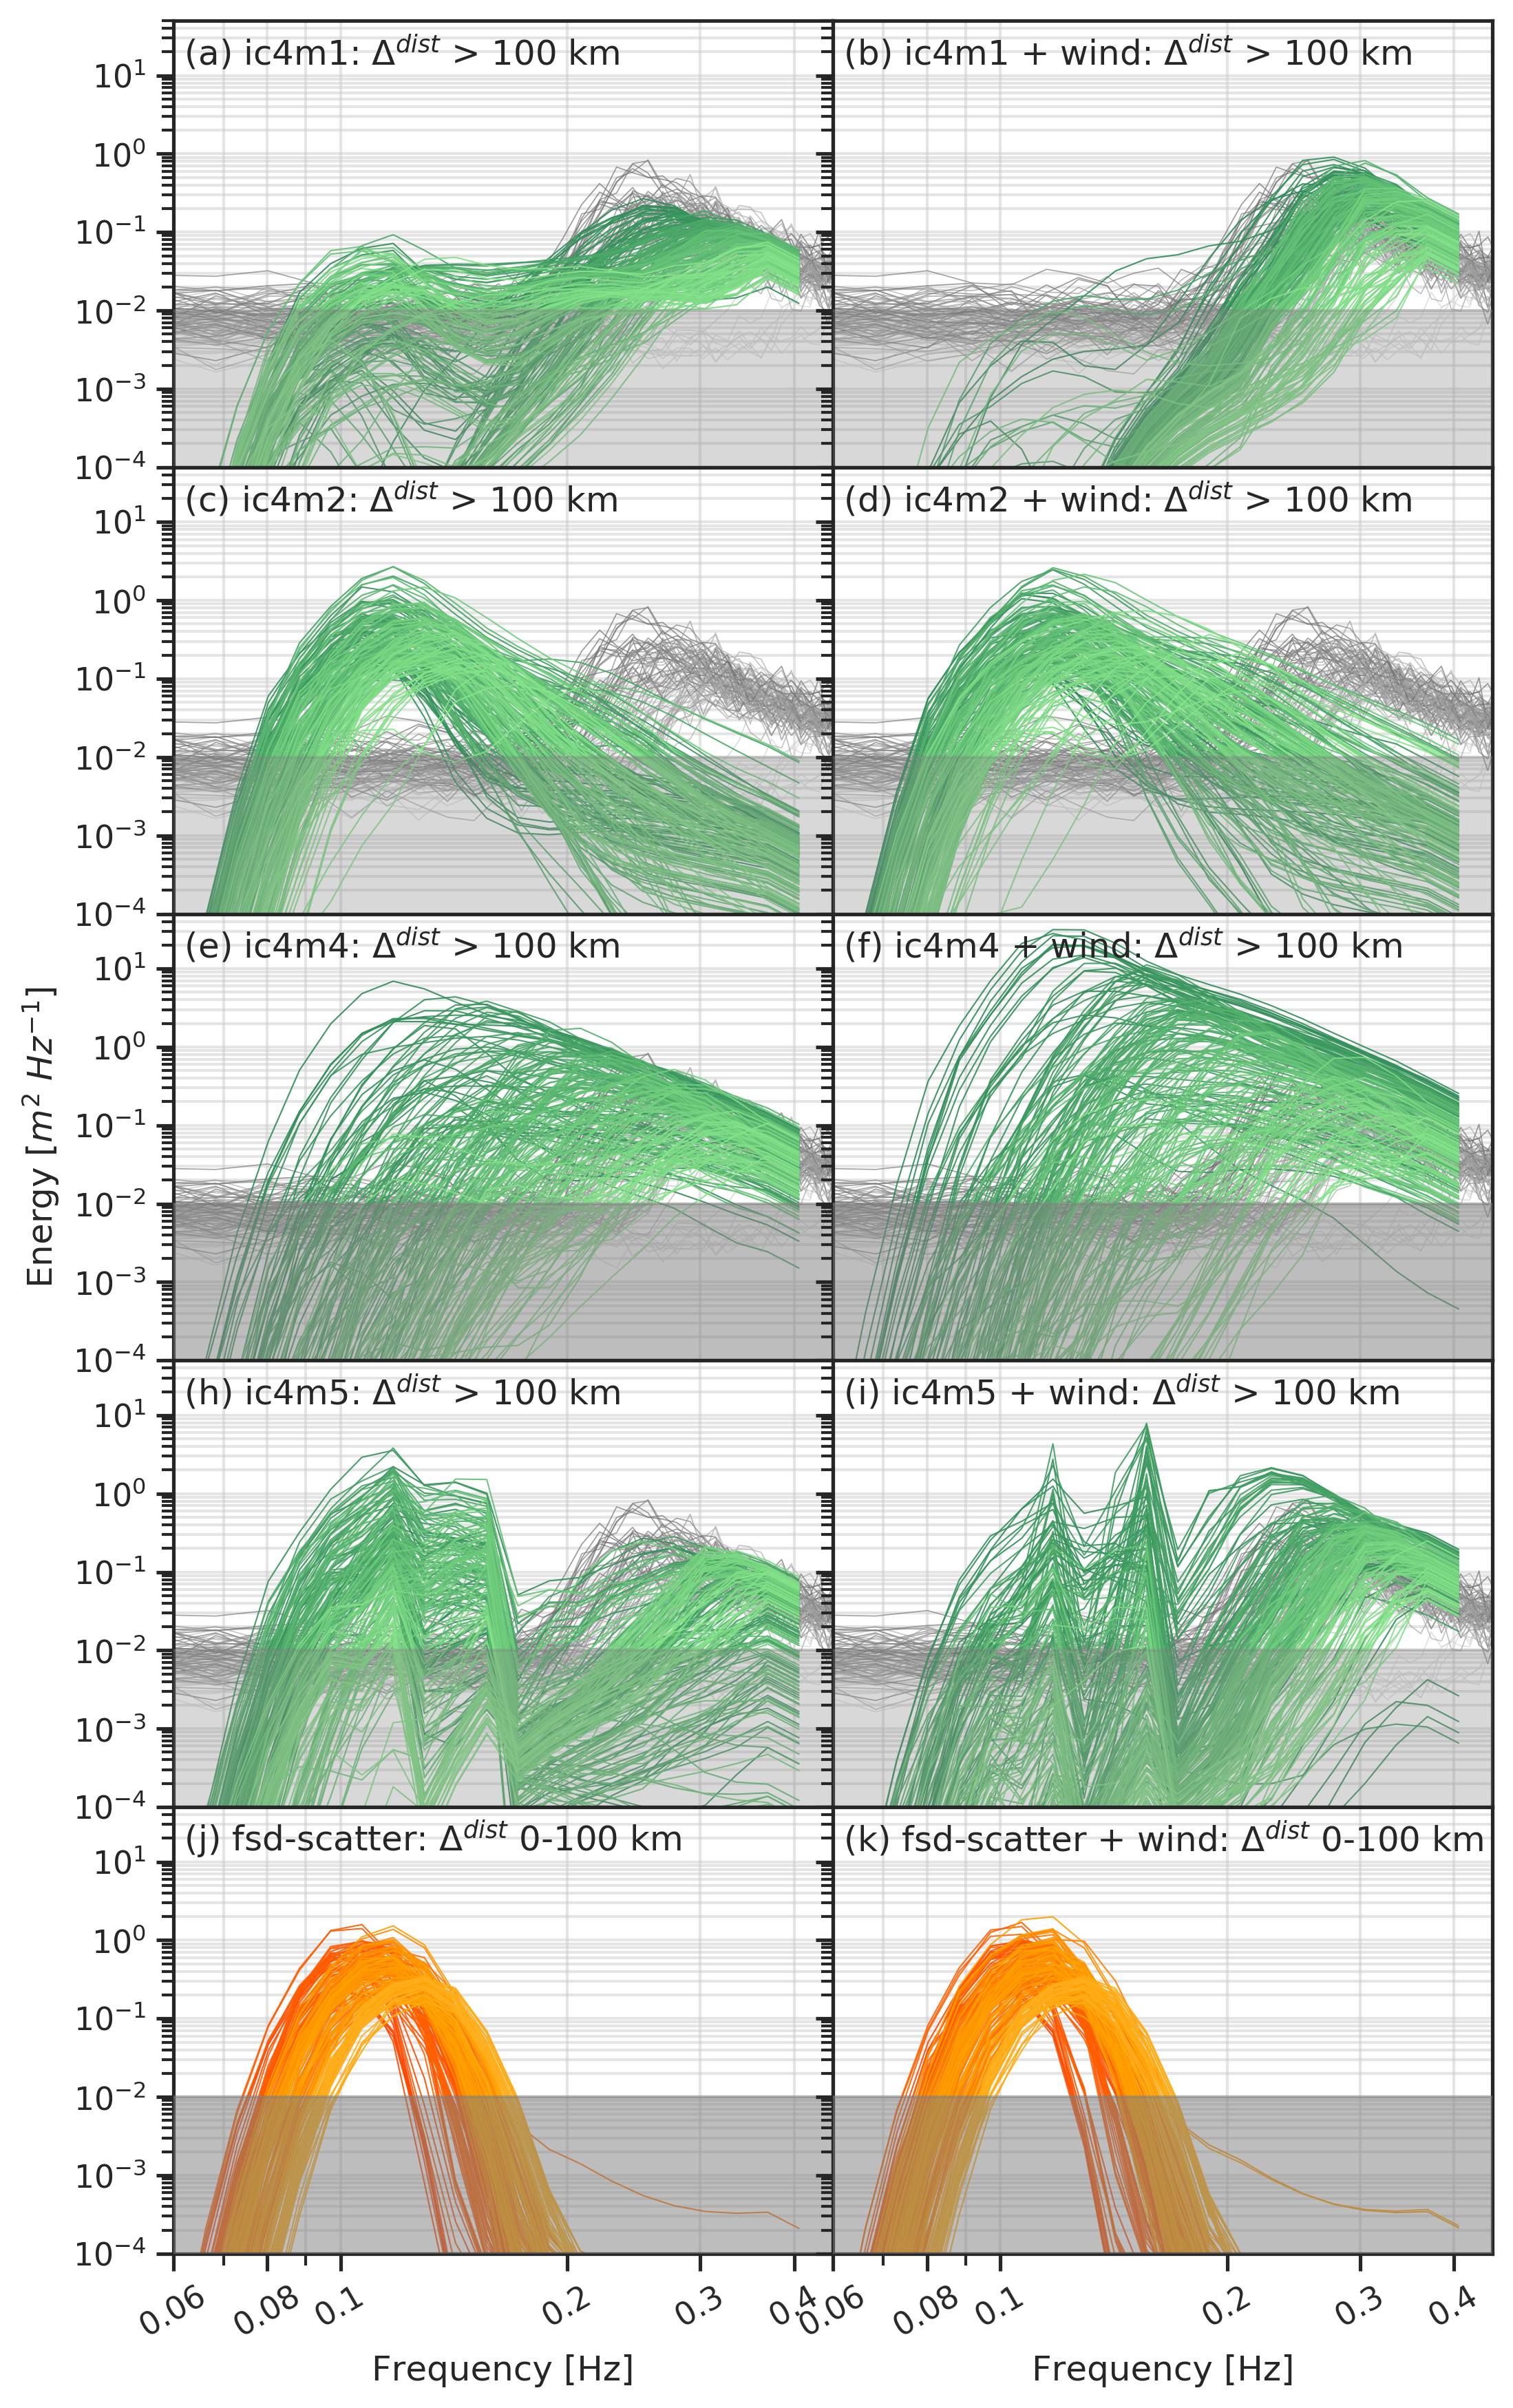
\includegraphics[height=0.72\textheight]{model-spec_04.png}
    \caption{
    Hourly-mean wave spectra from coupled wave-ice model experiments (green/orange colors) during July 2018 in the central Beaufort region surrounding the BGOS-SODA observations (latitudes 72$\degree$N to 79$\degree$N, longitudes 165$\degree$W to 130$\degree$W, see Figure \ref{fig:distance}c). For visual clarity, plots show model spectra (colored by peak frequency) from only 200 randomly selected grid cells when $H_s$ is greater than 0.3 m. Each row is a different attenuation scheme corresponding to Table \ref{tab:experiments}. Left column represents the standard experiment setup (wind input declining to zero as SIC approaches 100\%). Right column represents experiments with additional wind input (wind input declining to 50\% as SIC approaches 100\%). Bottom panels j-k (orange colors) show first 0-100 km because there are no model spectra with $H_s$ $>$ 0.3 m beyond 100-km $\Delta^{ \mathrm{dist}}$ in the FSD-scatter case. BGOS-SODA observations from July (all years) beyond 100 km are shown in grey. No observations are available in July from the first 0-100 km (j-k). Grey shading below $10^{-2}$ represents approximate detection limit of BGOS-SODA instruments, included for reference. Results are not sensitive to the random sampling of spectra (SI Figure \ref{SI:model-spec-alt}).}
    \label{fig:model-spec}
\end{SCfigure}

%Can experiments in a global coupled wave-ice model reproduce the observed wind-wave spectra inside the ice edge?
We now investigate how variations in wave-ice physics influence the simulation of ocean surface waves in the presence of sea ice, with particular attention to reproducing the spectral shape of observed wind waves in partial ice (Figure \ref{fig:obspanel}f). Figure \ref{fig:model-spec} shows model results from the central Beaufort Sea during July, the month when the vast majority of wind-wave observations at 100+ km $\Delta^{ \mathrm{dist}}$ in BGOS-SODA occur (SI Figure \ref{SI:months}c). Experiments IC4M3rad1 and IC4M7 have no spectra with $H_s$ greater than 0.1 m where SIC exceeds 15\% in July 2018, so these experiments are omitted from Figure \ref{fig:model-spec}.  

We first focus on the high-frequency portion of the spectrum. Across the model experiments, IC4M1 (Figure \ref{fig:model-spec}a-b) agrees most closely with the Beaufort Sea observations (Figure \ref{fig:obspanel}f) in that its dominant wave mode at 100+ km $\Delta^{ \mathrm{dist}}$ is the short wind waves. The agreement with observations is particularly strong in the experiment that allows substantial wind input even when SIC is high (Figure \ref{fig:model-spec}b). Notably, IC4M1 is neither new nor complex. It is a simple exponential function of period based on field experiments published in 1988 \cite{Wadhams1988TheZone}. IC4M5 also has a clear wind-wave spectral signature in the high-frequencies (Figure \ref{fig:model-spec}h-i). The FSD-scatter experiments damp all $H_s$ to less than 0.3 m before the waves reach 100-km $\Delta^{ \mathrm{dist}}$ (not shown), but the spectra from the first 0-100 km demonstrate that high-frequency energy is eliminated rapidly in ice (Figure \ref{fig:model-spec}j), and that allowing additional wind input does not change the story (Figure \ref{fig:model-spec}k). The results for IC4M3rad1 and IC4M7, which both depend on ice thickness, have even stronger damping than FSD-scatter (not shown).  

Turning to the low-frequency portion of the spectrum, many of the models appear to have too much low-frequency energy at 100+ km $\Delta^{ \mathrm{dist}}$ compared to observations. IC4M1 is a notable exception in that its spectra at 100+ km $\Delta^{ \mathrm{dist}}$ show lower levels of swell. IC4M2, M4, and M5 all have much higher energy in the low-frequency range than we see in observations. Note that spectra from M5 show abrupt jumps in energy because $\alpha$ is a piecewise (not smooth) function in that case (SI Figure \ref{SI:alpha}). FSD-scatter also favors the low-frequencies, showing swell spectra at 0-100 km $\Delta^{ \mathrm{dist}}$ that have similarities with some observations in Figure \ref{obs-results}h, although most of those observations are from October rather than July (SI Figure \ref{SI:months}b).    

In summary, the different attenuation schemes produce a wide range of spectral shapes in the July 2018 Beaufort Sea. A weak high-frequency attenuation rate (e.g. IC4M1 and IC4M5) permits the development of local wind waves beyond 100-km $\Delta^{ \mathrm{dist}}$ that resemble the observations, with the simple scheme of IC4M1 most closely resembling the observed spectra.  



\section{Simulated Wave-affected Extent Across Polar Oceans} \label{model-waveextent}

%Having considered the simulated spectra in the Beaufort Sea, we next test whether differences between attenuation schemes and additional wind input have an impact on the wave climate in sea ice across the polar oceans. While the BGOS-SODA observations are confined to the western Arctic, we would like to consider---using the coupled model---how uncertainty in wave-ice physics affects all regions where waves meet sea ice. We expect substantial seasonality in wave activity at least from (i) wintertime sea ice extent increasing how much ice is available for wave impacts and (ii) weather conditions, e.g. elevated autumn/winter storm activity. Figure \ref{fig:model-wave} shows that changing the magnitude and structure of the attenuation rate has a substantial impact on how much sea ice is subjected to wave activity in all seasons, and this sensitivity is present in both hemispheres. Seasonality in wave activity is generally consistent across hemispheres, and the amplitude of each seasonal cycle is sensitive to changes in wave-ice physics.  

Having compared models and observations in the western Arctic, we next investigate how uncertainty in wave-ice physics impacts the wave climate in sea ice globally. Our aim here is to explore the spatial extent of wave-ice interactions in the Arctic and Antarctic, and consider differences across hemispheres and seasons. We define the wave-affected extent as the total ocean area with SIC greater than 15\% and $H_s$ greater than 0.3 m (the threshold of detection that is applied in the BGOS-SODA observations). The spread in wave-affected extent between the attenuation schemes is substantial in both the Northern and Southern Hemispheres (Figure \ref{fig:model-wave}).  

In the Arctic (Figure \ref{fig:model-wave}a,b), schemes with the strongest attenuation result in a near-zero wave-affected extent during part of the summer season. Weaker attenuation rates yield nontrivial wave-affected extents even in the summer. The additional wind input (Figure \ref{fig:model-wave}b) has a major impact on the weakest attenuation rates---more than doubling the wave extent for IC4M4 and IC4M5---but the schemes with strong damping of high-frequency energy are relatively unaffected. IC4M1 (which most closely resembles BGOS-SODA observations in the Beaufort Sea) shows a substantial increase in wave-affected extent when wind input is enhanced.  

\begin{figure}
    \noindent\includegraphics[width=1.0\textwidth]{modelwave_03.png}
    \caption{2018 monthly mean of daily wave-affected extent (solid lines) and sea ice extent (dashed lines) in global coupled wave-ice model experiments. (a-b) Northern Hemisphere and (c-d) Southern Hemisphere. Left column represents the standard experiment setup (wind input declining to zero as SIC approaches 100\%). Right column represents experiments with additional wind input (wind input declining to 50\% as SIC approaches 100\%). Colored shading represents $\pm 1$ standard deviation of the daily wave-affected extent computed for each month.}
    \label{fig:model-wave}
\end{figure}

In the Southern Hemisphere (Figure \ref{fig:model-wave}c,d), the spread between the schemes is enhanced compared to the Arctic. During the summer minimum ice extent, the wave extents are spread between near-complete coverage of all sea ice (IC4M4) and near-zero wave extent (IC4M7). All methods besides IC4M7 have substantial wave-affected extent throughout most of the year. IC4M2, IC4M3rad1, IC4M7, and FSD-scatter are relatively unaffected by the additional wind input in Figure \ref{fig:model-wave}d, while IC4M1, IC4M4, and IC4M5 experience substantial increases in wave extent from the wind input, but mostly during the colder months. IC4M1 has a relatively small wave extent compared to the other attenuation schemes even when supplied with additional wind input. IC4M3 has relatively large wave extent in the Antarctic winter compared to the other schemes, whereas it has a relatively small wave extent in the Arctic winter.  

%In summary, the spread in wave-affected extent between the attenuation schemes is substantial. Additional wind input in ice increases the spread. While some attenuation schemes produce a consistently smaller/larger wave extent both hemispheres, other attenuation schemes (e.g. IC4M1 and IC4M3rad1) have contrasting relative performance in the Northern and Southern Hemispheres.  

% ========== Chapter 4
\chapter{Discussion} \label{discussion}

% wind waves exist in obs
Analysis of the BGOS-SODA observations reveals high-frequency wind waves beyond 100-km $\Delta^{\mathrm{dist}}$. In Figure \ref{fig:fetch-frac}a, we calculate the implied fetch for each wind-wave spectrum in BGOS-SODA observations according to the fetch-limited scaling relations (as described in Appendix \ref{scaling-method}, following \cite{Young1999}). The implied fetch can be estimated from either the nondimensional energy $E$ or frequency $F$---differences between the estimates result from scatter around the power law in Figure \ref{fig:obspanel}i. Both estimates suggest that all observed wind waves from beyond 100-km $\Delta^{\mathrm{dist}}$ require less than 50 km of open water fetch, and the majority of measurements require less than 20 km. SAR imagery from 18 July 2018 (Figure \ref{fig:SAR}a) provides an example illustrating small open water patches within relatively compact sea ice. Small wind waves could arise in these open water areas just as short waves develop in lakes. Wind waves were indeed reported by both BGOS-D and BGOS-A on July 20.  

\begin{figure}
    \noindent\includegraphics[width=0.99\textwidth]{fetch-frac_03.png}
    \caption{(a) Implied fetch for locally generated wind waves from BGOS-SODA mooring observations at 100+ km $\Delta^{ \mathrm{dist}}$, based on nondimensional frequency $F$ versus nondimensional energy $E$. 50x50 km size of axes corresponds to model grid resolution in central Beaufort Sea. (b) Observed spectra from BGOS-SODA at 100+ km $\Delta^{ \mathrm{dist}}$ (25th percentile, 75th percentile, and 99th percentile based on $H_s$) interpolated to the frequency domain used in model simulations. Grey shading represents approximate detection limit of instruments. (c) Histograms of predicted floe size distributions resulting from fracture by corresponding wave spectra in (b), based on the \cite{Horvat2015} parametrization, assuming ice thickness of 0.5 m. Floe sizes in panel c are binned into probability distributions $A(r)$ where $A(r)dr$ is the fraction of ice area with floe radius between $r$ and $r + dr$. Plots show the probability $A(r_i)dr_i$ at each of the following bin centers $i$: 3, 10, 22, 41, 70, 114, 176, 260, 370, 506, 668, and 850 m. Red line at radius of 15 m is provided as reference for limit at which lateral melt has been suggested to be significant \cite{Steele1992SeaModel}.}
    \label{fig:fetch-frac}
\end{figure}

\begin{figure}
    \noindent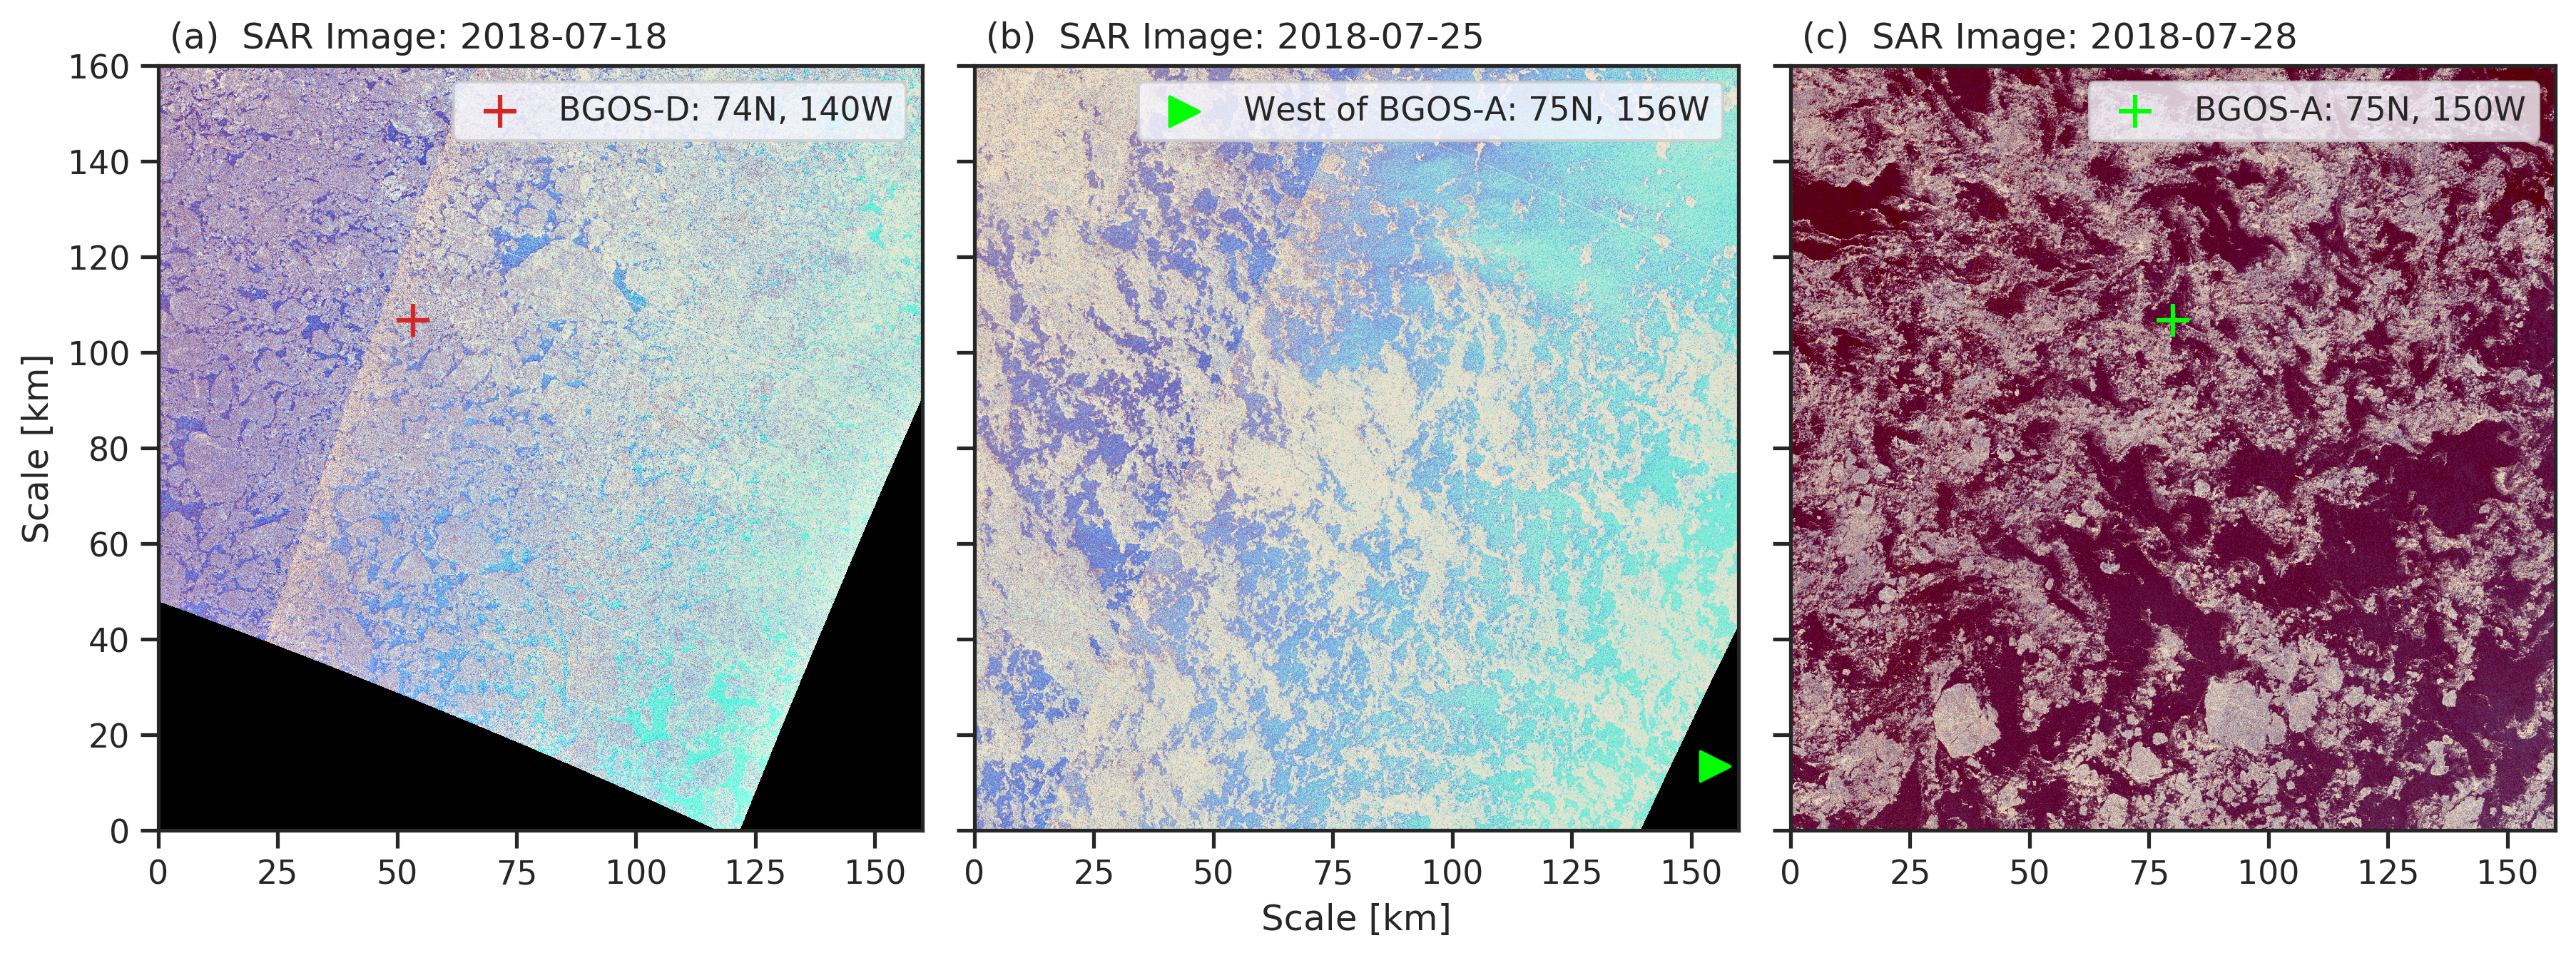
\includegraphics[width=0.99\textwidth]{SAR_02.png}
    \caption{SAR imagery in the Beaufort Sea on (a) 18 July 2018 located over BGOS-D (and east of BGOS-A), (b) 25 July 2018, from west of BGOS-A, and (c) 28 July 2018, located over BGOS-A. Sea ice shown in off-white colour \cite{SentinelHubEOBrowser, RaspaudSAR-Ice:Composite}.}
    \label{fig:SAR}
\end{figure}

% in spite of resolution limitations, can simulate them in the model
The estimated fetch required for the observed wind waves is shorter than the model grid resolution of approximately 50 km (Figure \ref{fig:fetch-frac}a). Despite this coarse resolution, existing attenuation schemes in WW3, especially IC4M1, can produce local wind waves in ice. WW3 is not fully resolving the fetch-limited generation process in this situation, but rather the balance between wind input by $S_{in}$, attenuation by $S_{ice}$, and their respective scaling by SIC, results in wave spectra that match the local wind waves. The ability to simulate these waves is sensitive to both the attenuation scheme---especially due to the wide range of high-frequency attenuation rates (Table \ref{tab:experiments}, SI Figure \ref{SI:alpha})---and the amount of wind input in ice.  

% do they matter?
To test the importance of the observed high-frequency wind waves for floe fracture, we input the 25$^\mathrm{th}$ percentile, 75$^\mathrm{th}$ percentile, and 99$^\mathrm{th}$ percentile wave spectra, ranked by \(H_s\), from BGOS-SODA observations beyond 100-km $\Delta^{\mathrm{dist}}$ to the \cite{Horvat2015} fracture parameterization (denoted HT15, computed offline). Given the wave spectrum, HT15 generates realizations of the sea surface height, computes the strain applied to sea ice floes, and returns a distribution of fractured floe sizes from the locations where the strain field exceeds a critical value. Figure \ref{fig:fetch-frac}c shows the resulting floe size distributions that would be formed by the observed wave spectra in Figure \ref{fig:fetch-frac}b with a representative ice thickness of 0.5 m. The HT15 parametrization suggests that locally generated waves at 100+ km $\Delta^{\mathrm{dist}}$ are strong enough to fracture sea ice. The 25$^\mathrm{th}$ percentile $H_s$ spectrum reduces 71\% of the ice area to floes with radius less than 15 m (Figure \ref{fig:fetch-frac}c), the floe radius below which lateral melt plays a critical role in Arctic summer conditions \cite{Steele1992SeaModel}. Note that the vast majority of local wind wave observations at 100+ km $\Delta^{\mathrm{dist}}$ occur in July (SI Figure \ref{SI:months}) when summer melt is underway.  

%implications for modelling
However, in coupled wave-ice model experiments using the HT15 fracture parameterization that show local wind wave spectra in the Beaufort Sea (e.g. IC4M1, Figure \ref{fig:model-spec}a,b), simulated floe sizes are unrealistically small across the polar oceans---IC4M1 has mean floe radius of 15 m (Arctic) and 7 m (Antarctic) at the end of the experiment (not shown). The HT15 parameterization assumes the entire sea ice cover in a grid cell experiences a single wave spectrum and is fractured accordingly. When considering subgrid-scale wind waves, which could be generated over a 10-km fetch and then attenuated rapidly in ice, it is likely incorrect to assume the all sea ice in a grid cell feels the immediate effect of the wind waves. Further work is required to validate and modify the floe fracture parameterization for locally-generated wind waves.  

In the SAR imagery from July 2018, the next image available after the onset of wind waves reported on July 20 (Figure \ref{fig:SAR}b, from July 25) shows substantial open water areas amid patchy sea ice cover. Three days later, Figure \ref{fig:SAR}c (located over BGOS-A on July 28) shows smaller floes and reduced SIC. Taken together, these images may indicate a melt event driven in part by local wind wave activity. The potential fracturing effect of locally generated wind waves---and their ability to enhance sea ice lateral melt---suggest that they should be a priority for future wave-ice model development.  

% \section{Swell waves}

We find little evidence for swell beyond 100 km inside the sea ice edge in the Beaufort Sea observations. However, the attenuation schemes that have waves inside the ice edge mostly have energy at low frequencies (Figure \ref{fig:model-spec}) rather than at high frequencies as shown in the observations (Figure \ref{fig:obspanel}f). We speculate that the low-frequency attenuation rate may need to be stronger than that of IC4M2, IC4M4, and IC4M5 to improve comparison with observations.  

Across the polar oceans, we find that changing the attenuation scheme can have substantial impacts on the areal extent of wave activity in sea ice (Figure \ref{fig:model-wave}). When the high-frequency attenuation of a given method is relatively weak, allowing additional wind input for wave generation in full ice cover also has a large impact on wave-affected extent. For some of the attenuation schemes (e.g. IC4M7, IC4M3rad1, FSD-scatter), the high-frequency damping is so strong in ice that the additional wind input still cannot overcome it.

Some attenuation schemes (e.g. IC4M1, IC4M3rad1) have different behavior in the Northern and Southern Hemispheres. This may be attributable to differences in the prevailing wave periods that arise in the Arctic ocean compared to the Southern Ocean. The Southern Ocean hosts much longer swells than the Arctic \cite{Liu2016WindAltimeters, Young2020TheOcean}. IC4M3rad1 has weak attenuation for the longest waves because it assumes a floe radius of 1 meter. While it damps waves effectively in the Arctic (Figure \ref{fig:model-wave}a,b), it has a relatively large wave extent in the Antarctic (Figure \ref{fig:model-wave}c). Increasing wind input in ice (Figure \ref{fig:model-wave}d) has no effect because the prevailing wave mode is swell propagating into ice from the open ocean, and IC4M3rad1's high-frequency attenuation is too strong to allow any wind waves in ice. IC4M1 illustrates a different situation: high-frequency attenuation is weak (SI Figure \ref{SI:alpha}), so wave extent is increased with wind input (Figure \ref{fig:model-wave}b,d). IC4M1 also has relatively strong attenuation for the long waves in the Southern Ocean, so it has a smaller wave-affected extent compared to other experiments in the Southern Hemisphere (Figure \ref{fig:model-wave}c,d).  

Our results suggest that constraining the attenuation rate of waves in ice requires further attention. They further highlight that understanding the balance of high-frequency attenuation and wind input in partial ice for local wind waves is also important, although this has received less attention in previous studies. The spectral properties of waves resulting from these processes and how they influence floe fracture will be important for understanding future sea ice evolution, particularly during the Arctic summer melt. We have not investigated the modulation of nonlinear transfer by sea ice, but this may represent another important and uncertain process that has a substantial effect on the shape of the wave spectrum.   

% ========== Chapter 5
 
\chapter{Conclusions} \label{conclusion}

In this study, we first investigate wave spectra in a multi-year dataset (BGOS-SODA) from five subsurface moorings in the Beaufort Sea under seasonal ice cover. Between the ice edge and 100 km inside it, the observations show waves with a range of peak frequencies, representing a mixture of wind waves and swell. Beyond 100 km, all observed spectra have significant wave heights less than 1 m. The vast majority (96 of 98 records) approximately follow the fetch-limited power law for local wind-wave generation. These small wind waves are generated over short distances (typically less than 20 km) in patches of open water amid partial ice cover. They may have a significant impact by breaking up sea ice into small floes (radius $<$ 15 m). These waves occur during the summer, mostly in July, and may therefore enhance lateral melt. However, future work is needed to understand to what extent high-frequency, local wind waves are able fracture sea ice and affect lateral melt.  

Secondly, we examine the impact of varying wave-ice physics, specifically wave attenuation and wind input in ice, in a global coupled wave-ice model. Focusing on the July 2018 Beaufort Sea and distances beyond 100 km from the ice edge, we find that most model experiments do not produce the short wind waves in ice seen in the BGOS-SODA observations. A weak high-frequency attenuation rate (as in the IC4M1 scheme) is required to simulate these local wind waves, and the agreement with observations is stronger when additional wind input is permitted in high concentrations of sea ice. Several attenuation schemes investigated here result in swell waves at large distances inside the sea ice edge, which are not supported by the BGOS-SODA observations. Globally, we find that changing the attenuation scheme has a remarkable effect on the wave-affected ice extent. Allowing wind input in full sea ice can have a pronounced impact, but only when the attenuation rate at high-frequencies is relatively weak.

The experiments demonstrate that the physics of wave-ice interactions require tighter constraints to provide a plausible simulation of the wave climate and floe size distribution across ice-covered oceans in a global model. We need more robust observations of floe sizes and wave spectra in sea ice across seasons and ocean basins. These observations would help constrain wave attenuation and generation in the marginal ice zone and wave effects on floe size, which are all critical to wave-ice model and theory development.  

\printendnotes

%

% ==========   Appendices
%
\appendix
\raggedbottom\sloppy
 
% ========== Appendix A
\chapter{Nondimensional Scaling for Wind-generated Ocean Waves} \label{scaling-method}

To interpret wave statistics, we employ nondimensional scaling for wind-generated waves following \cite{Young1999}. These relations enable separation of wind waves from swell and provide an estimate of the implied fetch for observed wind waves in partial ice cover. We calculate the following nondimensional variables for wave energy \(E\), frequency \(F\), and fetch distance \(X\):


\begin{align}\label{eq:nondim}
% \begin{split}
E = \left(\frac{g H_s}{4 U^2_{10}} \right)^2, \hspace{20pt} 
F = \frac{f_p U_{10}}{g}, \hspace{20pt}  
X = \frac{g x}{U^2_{10}},
% \end{split}
\end{align}

\noindent where \(g\) is the gravitational acceleration; \(U_{10}\) is the 10-meter wind speed at the location of each in situ observation and model grid cell from JRA-55 reanalysis \cite{KOBAYASHI2015TheCharacteristics, cisl_rda_ds628.0}; \(H_s\) is the significant wave height, defined as $4 \sqrt{ \int E(f)\,df}$; \(f_p\) is the peak frequency; and \(x\) is the fetch, i.e. the distance over which waves are generated by local winds. \(H_s\) and \(f_p\) are measured in situ and provided in model output. The fetch \(x\) is not measured but rather inferred for specific wind waves as described below; we refer to this variable as the implied fetch.  

In the marginal sea region of the observations considered, wave generation is generally limited by fetch rather than wind duration \cite{Hasselmann1973,Thomson2014SwellOcean}. Several studies have developed empirical estimates of power laws for \(E\) vs. \(X\) and \(F\) vs. \(X\) that describe wind-generated waves in a fetch-limited regime. \cite{Young1999} combined these estimates into the relations


\begin{equation}
E = \left(7.5 \pm 2.0 \right) \times 10^{-7} X^{0.8},
\label{eq:EvsX}
\end{equation}

\begin{equation}
F = \left(2.0 \pm 0.3 \right) X^{-0.25},
\label{eq:FvsX}
\end{equation}

\noindent which apply at least until reaching a fully developed limit for pure wind seas at $E_{max} = \left(3.6 \pm 0.9\right) \times 10^{-3}$ and $F_{min} = 0.13 \pm 0.02$. Using equation (\ref{eq:nondim}), we reformulate these power laws in terms of the variables available from measurements and modelling, \(E\) and \(F\):


\begin{equation}
E = \left(6.9 \pm 3.8 \right) \times 10^{-6} F^{-3.2}.
\label{eq:EvsF}
\end{equation}

We identify waves that are accurately described by fetch-limited local wind generation, i.e. wind waves, as those that fall within the uncertainty bounds of the line defined by the power law in equation (\ref{eq:EvsF}). If a spectrum has less energy \(E\) than predicted by the wind-wave power law for a given frequency \(F\), and it has a wave age greater than 1, we determine that the spectrum represents swell, i.e. long-period waves produced by nonlocal winds.  

Wave age, a nondimensional parameter $\frac{c}{U}$ defined by the ratio of the dominant phase speed $c_p$ to the wind speed $U_{10}$, can also distinguish swell from local wind waves. We treat $c_p = \frac{g}{2 \pi f_p}$ following the deep-water limit for surface gravity waves. When the wave age exceeds 1, waves travel faster than the winds. We note that wave age can be expressed in terms of $F$ using equation (\ref{eq:nondim}) such that $\frac{c}{U} = \left(2 \pi F\right)^{-1}$, and wave age is greater than 1 when $F$ is less than $\frac{1}{2\pi}$.  

Taking only the spectra that appear to be fetch-limited local wind waves, based on equation (\ref{eq:EvsF}) and wave age, we can calculate an implied fetch \(x\) corresponding to each wind-wave spectrum. This dimensional variable \(x\) is recovered by solving for the nondimensional \(X\) in equation (\ref{eq:EvsX}) based on the known energy \(E\), then using equation (\ref{eq:nondim}) to restore the dimension. The implied fetch is an estimate of the open water distance that would be required for local winds to generate a given wind-wave spectrum.  


% ========== Appendix B
\chapter{Wind Speed Estimates from the Equilibrium Range}
\label{u10-method}

Surface wind speed can be estimated from the equilibrium range in the high-frequency end of the wave spectrum (the ``spectral tail''). The equilibrium range is the portion of the wave spectrum where the source terms---wind input, nonlinear transfer, and dissipation---are balanced \cite{Phillips1985SpectralWaves}. We follow the methods from \cite{Thomson2013WavesP, Voermans2020EstimatingSpectra} that calculate a friction velocity $u_{\ast}$ by assuming $E(f) \propto u_{\ast} f^{-4}$, where $E$ is energy and $f$ is frequency. This process begins with:


\begin{equation}
E(f) = E_0 f^{-4},\mathrm{\ where \ }E_0 = \frac{4 g \beta I_p u_{\ast}} {(2 \pi)^3},
\label{eq:E_0}
\end{equation}
\noindent 
and we compute $E_0$ as the mean of $f^4 E(f)$ for the frequencies in the equilibrium range. The equilibrium range is identified as the 20 consecutive frequencies (all higher than $f_p$, up to a maximum of 0.5 Hz) that minimize standard error on the fit to $f^{-4}$. We require a minimum of 10 data points in the equilibrium range. $\beta$ is an empirical constant that is set to 0.009 based on results in \cite{Voermans2020EstimatingSpectra}. $I_p$ adjusts for directional spreading of waves and ranges from 1.9 (wide) to 3.1 (narrow) \cite{Juszko1995WindTheory} with a typical value of 2.5 \cite{Thomson2013WavesP}. For observations beyond 100-km $\Delta^{\mathrm{dist}}$, we use $I_p = 1.9$, expecting that directional spreading may be elevated in partial ice cover. For observations in open water, we use the typical value of $I_p = 2.5$.  

We then have an estimate of $u_{\ast}$ which we can relate to the 10-meter wind speed $U_{10}$ by assuming a logarithmic wind profile in the boundary layer: 

\begin{equation}
U(z) = \frac{u_{\ast}}{\kappa} \mathrm{ln} \left( \frac{z}{z_0} \right),
\label{eq:u10log}
\end{equation}
\noindent
with the von Karman constant $\kappa = 0.41$, $z = 10$ meters, and ocean surface roughness length $z_0$. This is assumed to follow the Charnock relation \cite{Charnock1955WindSurface},


\begin{equation}
z_0 =  \frac{\alpha u_{\ast}^2}{g},
\label{eq:z_0}
\end{equation}
\noindent
although the presence of ice may impact $z_0$, introducing some additional uncertainty. Following equation (16) in \cite{Voermans2020EstimatingSpectra}, $\alpha$ is determined by wave age according to:

\begin{equation}
\alpha =  0.14 \left( \frac{u_{\ast}}{c_p} \right)^{0.61},
\label{eq:charnock}
\end{equation}
\noindent
where $c_p$ is the phase speed at the peak frequency. With these assumptions, we can estimate $U_{10}$ from the $E(f)$ measured by BGOS-SODA subsurface moorings, which are located roughly 30-45 meters beneath the ocean surface.  

\chapter{Supplemental Information}\label{SI}
\addtocontents{toc}{\protect\setcounter{tocdepth}{0}}
\section{Separation of Ice Spectra from Surface Wave Spectra} \label{icespectra}

Deformed sea ice produces a ``red'' spectrum with under-ice topography exhibiting peak spectral variance primarily at low frequencies \cite{Rothrock1980GeometricIce}, whereas the surface gravity waves tend to have peak energy in the frequency range of 0.5 to 0.05 Hz, causing sea surface displacements with distinct spectra in that range. Calm waters and smooth ice both produce flat (``white'') spectra. If both ice and waves are present, moorings measure a superposition of both signals.  

The processing strategies for the mooring datasets make use of these different spectral shapes to identify and separate wave signals from sea ice. The postprocessed wave datasets from BGOS and SODA exclusively contain observations where the surface gravity wave signal is sufficiently strong to be considered a wave, determined by the spectral shape and the total energy in the frequency range of ocean surface waves. If the ice-draft signal is strong while the surface wave signal is weak, the instrument may be unable to produce a valid wave measurement. These instances where only ice draft is detected are excluded from the wave datasets considered here.  

\section{Attenuation Rates in Ice}
\begin{figure}[H]
    \noindent\includegraphics[width=1.0\textwidth]{alpha_01.png}
    \caption{Reproduced for reference from \cite{Collins2017ANRL/MR/7320179726} based on WW3 model code \cite{TheWAVEWATCHIIIRDevelopmentGroupWW3DG2016User5.16}. Displays the frequency-dependent attenuation rate $\alpha$ of waves in ice used for various experiments corresponding to Table \ref{tab:experiments}. For some cases, parameters specified in Table \ref{tab:experiments} change the $\alpha$ relative to the illustrative values shown here. This plot uses thickness of 0.5 m and, for the FSD-scatter scheme, a floe size of 100 m.}
    \label{SI:alpha}
\end{figure}

\section{SWIFT Surface Buoy Spectra}
\begin{figure}[H]
    \noindent\includegraphics[width=1.0\textwidth]{swift_01.png}
    \caption{Wave spectra from free-drifting surface buoys as a supplemental line of comparison. Color shading according to the peak frequency as visual aid. These measurements come from Surface Wave Instrument Floats with Tracking (SWIFTs) \cite{Thomson2012WaveDrifters} that were deployed for short periods of time during large wave events in the Beaufort-Chukchi Sea during the Oct-Nov 2015 Arctic Sea State campaign. The SWIFTs measure ocean surface velocities and infer wave energy spectra every hour using GPS tracking \cite{Herbers2012ObservingBuoys}. The SWIFTs do not sample data continuously over extended periods of time. Only $H_s$ greater than 0.3 m are shown, and the detection limit of the BGOS-SODA observations is marked with grey shading. Note that the SWIFTs have a much lower detection limit, i.e. they resolve the spectra at energy levels much lower than those resolved by the subsurface moorings.}
    \label{SI:swift}
\end{figure}

\section{Model Spectra in the Beaufort Sea}
\begin{figure}[H]
    \noindent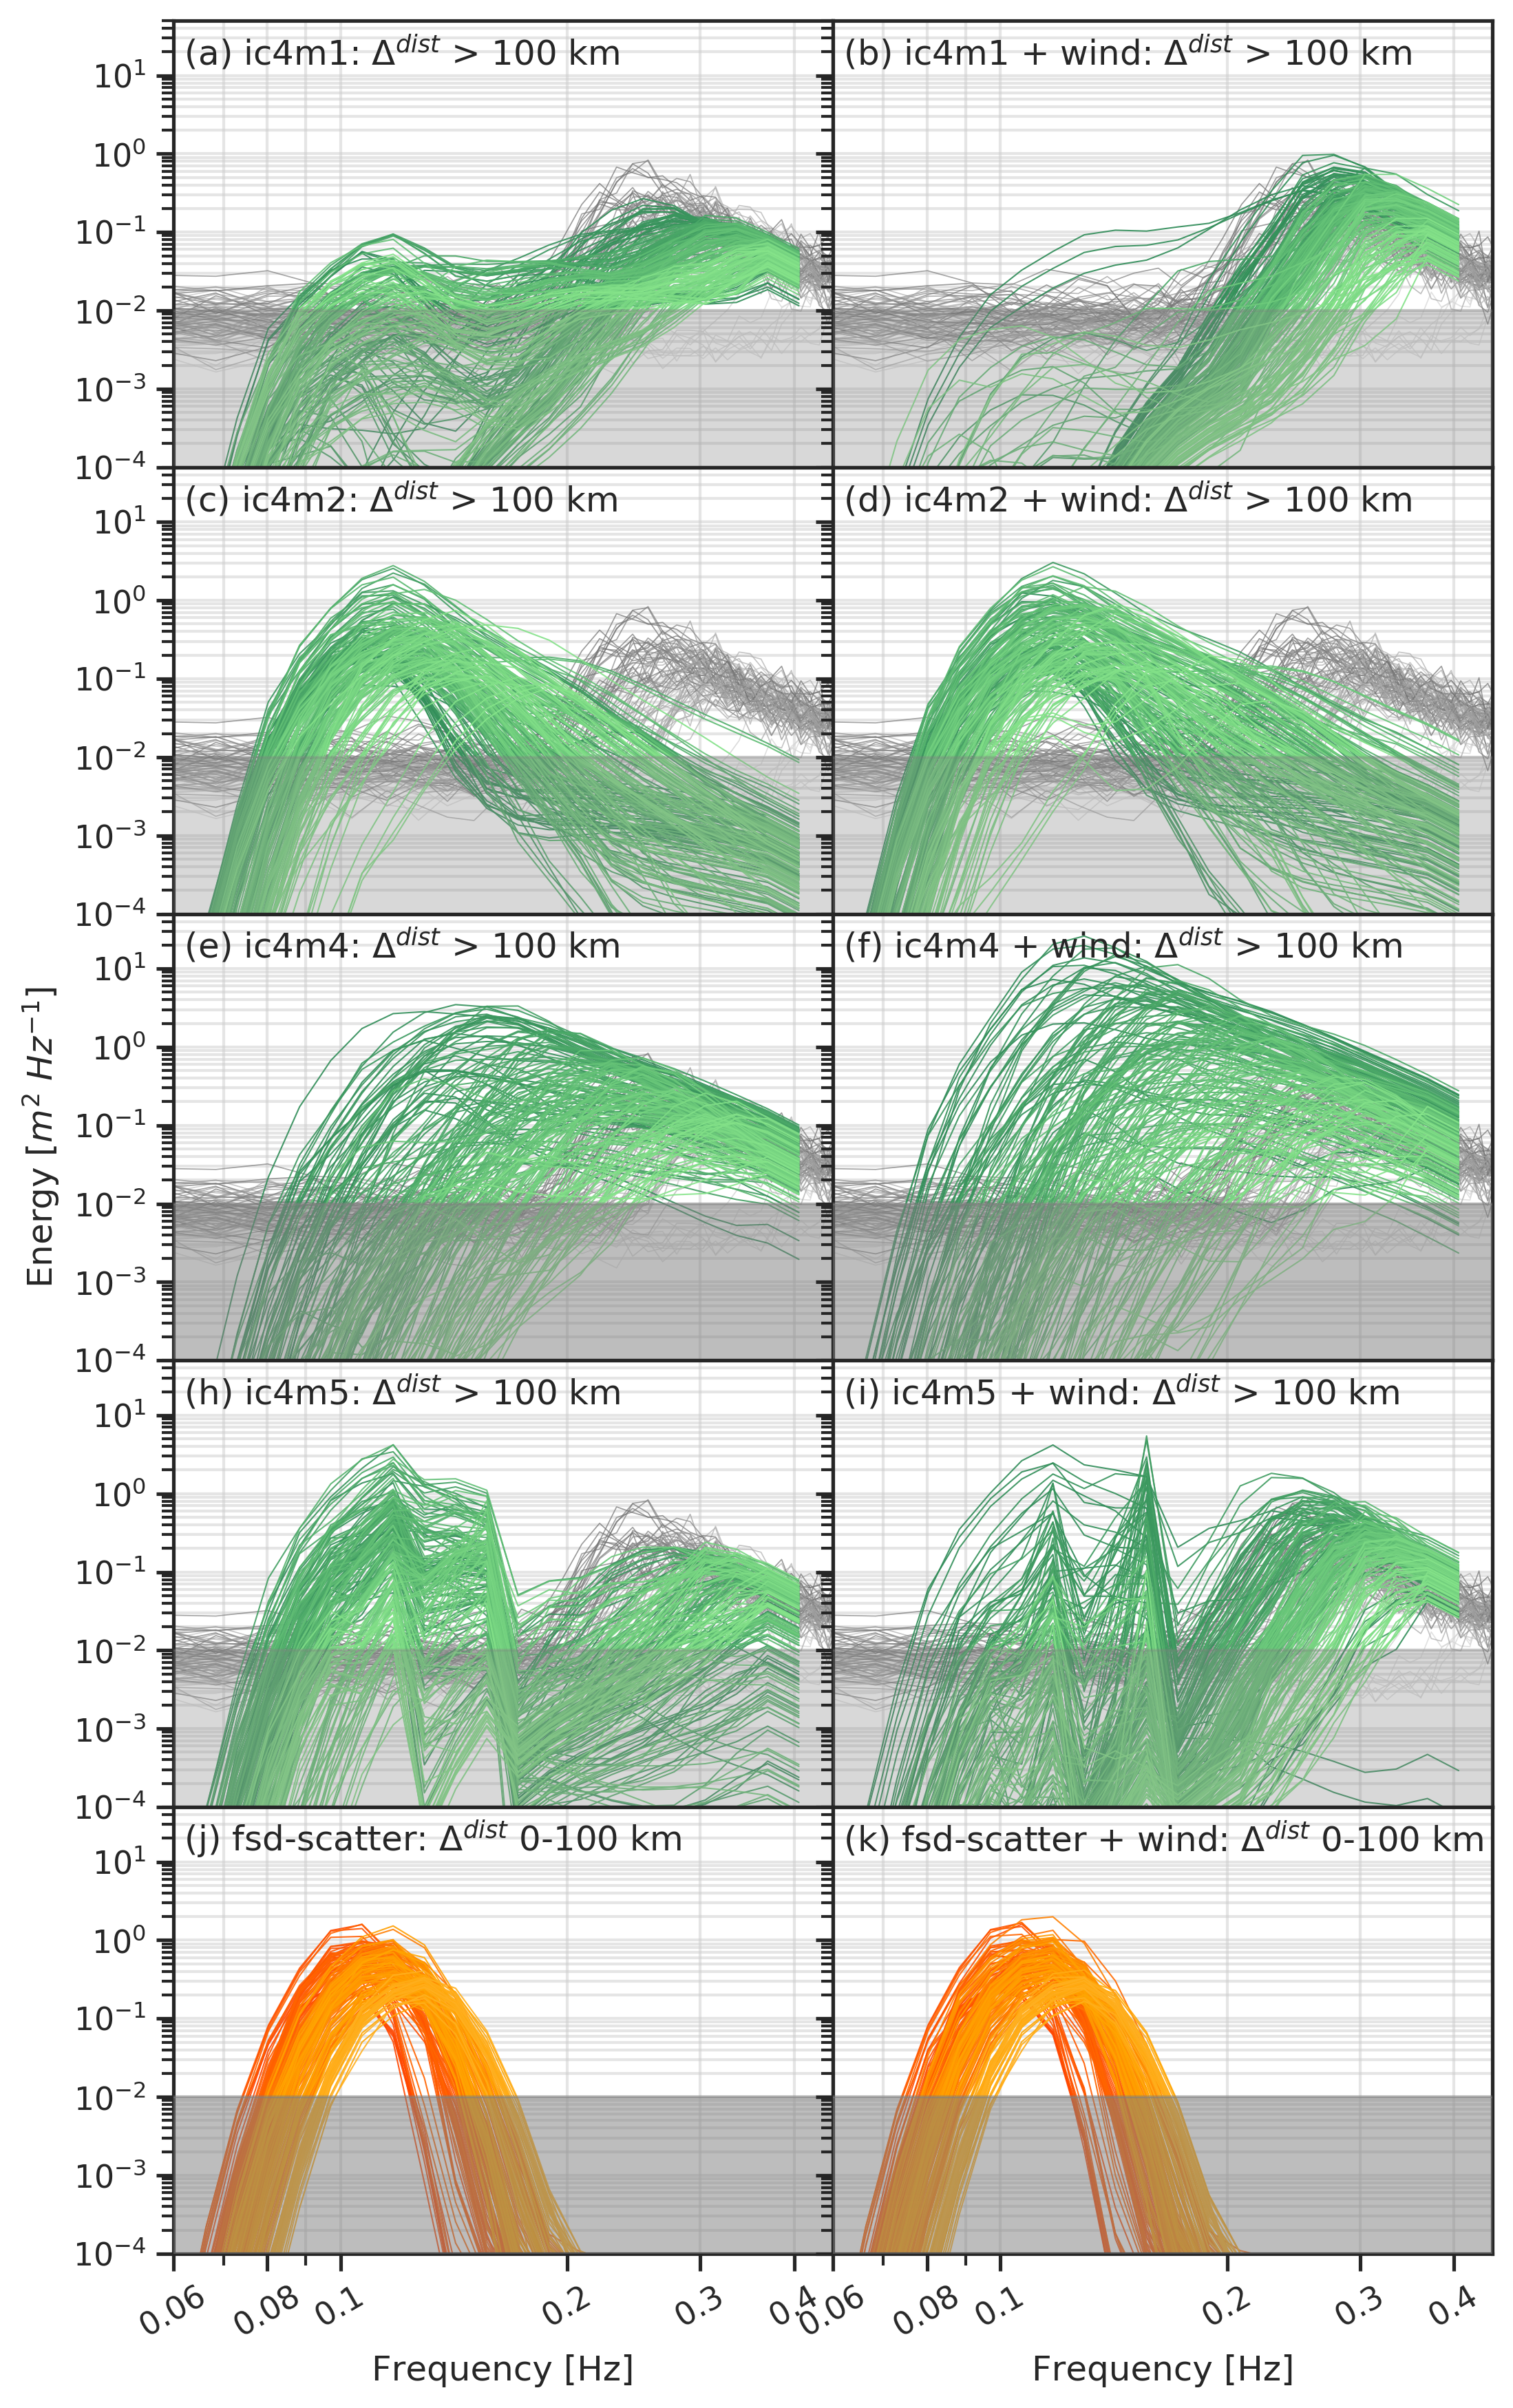
\includegraphics[height=0.8\textheight]{model-spec_04-altSI.png}
    \caption{A unique random sample of model spectra with description matching Figure \ref{fig:model-spec}.}
    \label{SI:model-spec-alt}
\end{figure}

\section{Timing of BGOS-SODA observations}
\begin{figure}[H]
    \noindent\includegraphics[width=1.0\textwidth]{months_02.png}
    \caption{Histogram of wave occurrence by month for significant wave height $>$ 0.3 m, spanning 2012-2021 and grouped by $\Delta^{\mathrm{dist}}$. Vertical axis represents the number of measurements coming from a given month.}
    \label{SI:months}
\end{figure}

% ==========   Bibliography
%
% \nocite{*}   % include everything in the uwthesis.bib file
% \bibliographystyle{plain}
% \bibliography{uwthesis}
\printbibliography[heading=bibintoc,title={Bibliography}]


\end{document}
